\documentclass[11pt,a4paper]{article}
\usepackage[T1]{fontenc}
\usepackage[utf8]{inputenc}
\usepackage{lmodern}
\usepackage{textcomp}
\usepackage[left=1.8cm,right=1.8cm,top=2.3cm,bottom=2.2cm,headheight=14pt,headsep=8pt]{geometry}
\usepackage{multicol}
\usepackage{xcolor}
\usepackage{fancyhdr}
\usepackage{graphicx}
\usepackage{array}
\usepackage{amsmath,amssymb}
\usepackage{setspace}
\usepackage{longtable}
\graphicspath{{../}}
\definecolor{ygreen}{RGB}{46,139,87}
\renewcommand{\normalsize}{\fontsize{10.9}{13.4}\selectfont}
\renewcommand{\familydefault}{\rmdefault}
\setlength{\parindent}{0pt}
\setlength{\columnsep}{0.8cm}
\setlength{\columnseprule}{0.4pt}
\setlength{\multicolsep}{3pt plus 1pt minus 1pt}
\renewcommand{\textsubscript}[1]{\ensuremath{_{\text{\fontsize{8}{8}\selectfont #1}}}}
\renewcommand{\textsuperscript}[1]{\ensuremath{^{\text{\fontsize{8}{8}\selectfont #1}}}}
\newcommand{\qn}[1]{\textbf{\fontsize{11.5}{13}\selectfont #1}}
\newcommand{\qsep}{\par\vspace{1pt}\noindent\rule{0pt}{0.4pt}\par\vspace{5pt}}
\newcommand{\fwrule}{\par\vspace{5pt}\noindent\rule{\linewidth}{1.4pt}\par\vspace{7pt}}
\newsavebox{\fitb}
\newcommand{\fitbox}[1]{\sbox{\fitb}{#1}\ifdim\wd\fitb>\linewidth\resizebox{\linewidth}{!}{\usebox{\fitb}}\else\usebox{\fitb}\fi}
\newcommand{\diqqat}[1]{\par\smallskip\noindent\textbf{Diqqat!} #1\par\medskip}
\newcommand{\javob}{\par\smallskip\noindent\textbf{Javob:} \rule[-2pt]{7.5cm}{0.4pt}\par\smallskip\noindent\textbf{Diqqat!} Javobingizni javoblar varaqasiga ko`chirib yozing.\par\medskip}
\pagestyle{fancy}
\fancyhf{}
\renewcommand{\headrulewidth}{0.4pt}
\fancyhead[L]{\textit{Milliy sertifikat 2026. Kimyo}}
\fancyhead[R]{11-variant}
\fancyfoot[L]{\fontsize{8}{9}\selectfont \textcopyright{} Colba maktabi, 2026}
\fancyfoot[C]{\thepage}
\fancypagestyle{first}{\fancyhf{}\renewcommand{\headrulewidth}{0pt}\fancyfoot[L]{\fontsize{8}{9}\selectfont \textcopyright{} Colba maktabi, 2026}\fancyfoot[C]{\thepage}}
\begin{document}
\normalsize
\thispagestyle{first}
\noindent\fcolorbox{ygreen}{white}{\parbox{\dimexpr\linewidth-2\fboxsep-2\fboxrule\relax}{%
\textbf{\fontsize{13}{15}\selectfont Nazorat testi}\ \textit{\fontsize{10}{12}\selectfont $\cdot$ Aralash test $\cdot$ 11-variant}\hfill
\begin{tabular}[t]{@{}r@{}}\textit{Milliy sertifikat 2026. Kimyo}\\ \textbf{\textit{\fontsize{8}{9}\selectfont Vaqt:}} \textit{\fontsize{10}{12}\selectfont 180 daqiqa}\end{tabular}}}
\par\medskip
\noindent\textit{Davriy jadvaldan foydalanish mumkin.}
\par\medskip
\begin{multicols}{2}
\noindent\qn{1.} 19,5 g Zn va 4,8 g S aralashtirilib, reaksiya o`tkazildi (Zn + S $\to$ ZnS). Hosil bo`lgan ZnS \textbf{massasini (g) aniqlang.}

\noindent A)~\textsl{14,55} \hfill B)~\textsl{29,1} \hfill C)~\textsl{7,27} \hfill D)~\textsl{21,82}\par
\qsep
\noindent\qn{2.} 28,6 g Na\textsubscript{2}CO\textsubscript{3}$\cdot$10H\textsubscript{2}O 300 g suvda eritildi. Eritmadagi tuzning massa \textbf{ulushini (\%) aniqlang.}

\noindent A)~\textsl{3,53} \hfill B)~\textsl{8,7} \hfill C)~\textsl{3,23} \hfill D)~\textsl{6,45}\par
\qsep
\noindent\qn{3.} Quyidagi jadvalda MgSO\textsubscript{4} tuzining eritmalari keltirilgan:
\begin{center}
\renewcommand{\arraystretch}{1.15}
\fitbox{\begin{tabular}{|c|c|c|}\hline
\textbf{No.} & \textbf{m(eritma), g} & \textbf{$\omega$, \%} \\ \hline
I & 150 & 20 \\ \hline
II & 100 & 30 \\ \hline
\end{tabular}}
\end{center}
Eritmalar aralashtirildi. Oxirgi eritmadagi tuzning massa \textbf{ulushini (\%) toping.}

\noindent A)~\textsl{24} \hfill B)~\textsl{25} \hfill C)~\textsl{50} \hfill D)~\textsl{26}\par
\qsep
\noindent\qn{4.} Jadvalda bog`lar hosil qiluvchi atomlarning elektrmanfiyliklari berilgan:
\begin{center}
\renewcommand{\arraystretch}{1.15}
\fitbox{\begin{tabular}{|c|c|c|}\hline
\textbf{Bog`} & \textbf{EM (1-atom)} & \textbf{EM (2-atom)} \\ \hline
Mg--O & 1,2 & 3,5 \\ \hline
H--F & 2,1 & 4 \\ \hline
Si--O & 1,8 & 3,5 \\ \hline
C--H & 2,5 & 2,1 \\ \hline
\end{tabular}}
\end{center}
Qaysi bog` eng qutbli (eng ko`p ionli xarakterga ega)?

\noindent A)~\textsl{H--F} \hfill B)~\textsl{Si--O} \hfill C)~\textsl{Mg--O} \hfill D)~\textsl{C--H}\par
\qsep
\noindent\qn{5.} 1 mol C\textsubscript{2}H\textsubscript{6} tarkibidagi atomlar \textbf{sonini toping} (N\textsubscript{A} = 6,02$\cdot$10\textsuperscript{23}). Javobni 10\textsuperscript{23} birligida yozing.

\noindent A)~\textsl{9,632} \hfill B)~\textsl{2,408} \hfill C)~\textsl{4,816} \hfill D)~\textsl{0,602}\par
\qsep
\noindent\qn{6.} Na\textsubscript{2}CO\textsubscript{3}$\cdot$10H\textsubscript{2}O kristallogidratida kristallizatsion suvning massa \textbf{ulushini (\%) aniqlang.}

\noindent A)~\textsl{37,1} \hfill B)~\textsl{62,9} \hfill C)~\textsl{31,5} \hfill D)~\textsl{169,8}\par
\qsep
\noindent\qn{7.} ZnSO\textsubscript{4} ning suvli eritmasi inert elektrodlar bilan elektroliz qilinganda qaysi moddalar ajraladi?

\noindent\begin{tabular}{@{}p{0.47\linewidth}@{}p{0.47\linewidth}@{}}
A)~\textsl{Zn, H\textsubscript{2} va O\textsubscript{2}} & B)~\textsl{H\textsubscript{2}, Cl\textsubscript{2} va NaOH} \\
C)~\textsl{Cu va Cl\textsubscript{2}} & D)~\textsl{Ag va O\textsubscript{2}} \\
\end{tabular}\par
\qsep
\noindent\qn{8.} Massa soni 226, zaryadi 88 bo`lgan yadro massa soni 206, zaryadi 82 bo`lgan yadroga aylandi ($\alpha$ va $\beta$\textsuperscript{$-$} parchalanish). Nechta $\beta$\textsuperscript{$-$}-zarra chiqarilgan?

\noindent A)~\textsl{5} \hfill B)~\textsl{3} \hfill C)~\textsl{4} \hfill D)~\textsl{6}\par
\qsep
\noindent\qn{9.} Quyidagi tuzlarning qaysilari suvli eritmasi ishqoriy muhitga ega? 1) K\textsubscript{3}PO\textsubscript{4}; 2) K\textsubscript{2}S; 3) Al\textsubscript{2}(SO\textsubscript{4})\textsubscript{3}; 4) NaCl

\noindent A)~\textsl{1} \hfill B)~\textsl{4} \hfill C)~\textsl{1, 2} \hfill D)~\textsl{1, 2, 3}\par
\qsep
\noindent\qn{10.} CH\textsubscript{3}--C$\equiv$CH molekulasida sp gibridlangan uglerod atomlari nechta?

\noindent A)~\textsl{3} \hfill B)~\textsl{4} \hfill C)~\textsl{1} \hfill D)~\textsl{2}\par
\qsep
\noindent\qn{11.} A elementi atomining ketma-ket ionlanish energiyalari diagrammada berilgan.
\begin{center}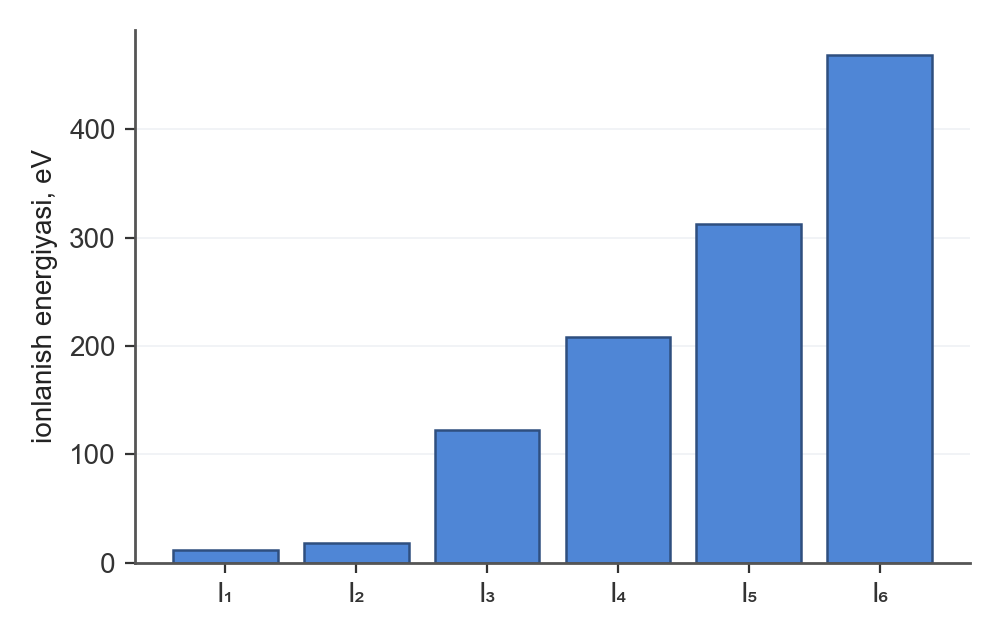
\includegraphics[width=0.86\linewidth]{rasmlar/gen/ie_v11_0.png}\end{center}
A elementining eng yuqori oksidi \textbf{formulasini toping.}

\noindent A)~\textsl{A\textsubscript{2}O} \hfill B)~\textsl{AO} \hfill C)~\textsl{A\textsubscript{2}O\textsubscript{3}} \hfill D)~\textsl{AO\textsubscript{2}}\par
\qsep
\noindent\qn{12.} Massa soni 238 va zaryadi 92 bo`lgan yadro massa soni 206, zaryadi 82 bo`lgan yadroga aylanishida nechta $\alpha$- va $\beta$\textsuperscript{$-$}-zarra chiqaradi?

\noindent A)~\textsl{8$\alpha$ va 6$\beta$} \hfill B)~\textsl{9$\alpha$ va 6$\beta$} \hfill C)~\textsl{8$\alpha$ va 8$\beta$} \hfill D)~\textsl{6$\alpha$ va 8$\beta$}\par
\qsep
\noindent\qn{13.} N\textsubscript{2}O\textsubscript{5} tarkibida azot ning \textbf{valentligini aniqlang.}

\noindent A)~\textsl{\textit{V}} \hfill B)~\textsl{VI} \hfill C)~\textsl{VII} \hfill D)~\textsl{IV}\par
\qsep
\noindent\qn{14.} Nodir gazlar haqida qaysi fikrlar to`g`ri? 1) Geliy eng yengil inert gaz; 2) Argon elektr lampalarida ishlatiladi; 3) Neon atomida 8 ta tashqi elektron bor; 4) Neon reklama naylarida ishlatiladi

\noindent\begin{tabular}{@{}p{0.47\linewidth}@{}p{0.47\linewidth}@{}}
A)~\textsl{1, 3, 4} & B)~\textsl{1, 2, 4} \\
C)~\textsl{1, 2, 3} & D)~\textsl{1, 2, 3, 4} \\
\end{tabular}\par
\qsep
\noindent\qn{15.} Zn(NO\textsubscript{3})\textsubscript{2} qizdirilganda qanday moddalar hosil bo`ladi?

\noindent\begin{tabular}{@{}p{0.47\linewidth}@{}p{0.47\linewidth}@{}}
A)~\textsl{NaNO\textsubscript{2} va O\textsubscript{2}} & B)~\textsl{ZnO, NO\textsubscript{2} va O\textsubscript{2}} \\
C)~\textsl{CuO, NO\textsubscript{2} va O\textsubscript{2}} & D)~\textsl{Ag, NO\textsubscript{2} va O\textsubscript{2}} \\
\end{tabular}\par
\qsep
\noindent\qn{16.} 2ZnS + 3O\textsubscript{2} $\to$ 2ZnO + 2SO\textsubscript{2} reaksiyasida tarkibida 75\% aralashma bo`lgan 77,6 g namuna (asosiy modda ZnS) ishtirok etdi. SO\textsubscript{2} \textbf{massasini (g) toping.}

\noindent A)~\textsl{25,6} \hfill B)~\textsl{6,4} \hfill C)~\textsl{19,2} \hfill D)~\textsl{12,8}\par
\qsep
\noindent\qn{17.} 42,5 g AgNO\textsubscript{3} to`liq parchalanguncha qizdirildi. Qattiq qoldiq \textbf{massasini (g) aniqlang.}

\noindent A)~\textsl{42,5} \hfill B)~\textsl{27} \hfill C)~\textsl{54} \hfill D)~\textsl{13,5}\par
\qsep
\noindent\qn{18.} 2CO + O\textsubscript{2} $\to$ 2CO\textsubscript{2} reaksiyasida 32 g O\textsubscript{2} ishtirok etdi (unum 80\%). CO\textsubscript{2} \textbf{hajmini (l, n.sh.) toping.}

\noindent A)~\textsl{11,2} \hfill B)~\textsl{35,84} \hfill C)~\textsl{71,68} \hfill D)~\textsl{17,92}\par
\qsep
\noindent\qn{19.} NaCl + AgNO\textsubscript{3} $\to$ AgCl + NaNO\textsubscript{3} jarayoni uchun 85 g AgNO\textsubscript{3} olingan. NaCl \textbf{massasini (g) aniqlang.}

\noindent A)~\textsl{58,5} \hfill B)~\textsl{14,62} \hfill C)~\textsl{43,88} \hfill D)~\textsl{29,25}\par
\qsep
\noindent\qn{20.} Reaksiya tenglamasi: C\textsubscript{3}H\textsubscript{8} + 5O\textsubscript{2} $\to$ 3CO\textsubscript{2} + 4H\textsubscript{2}O. Reaksiyaga 11,2 l (n.sh.) C\textsubscript{3}H\textsubscript{8} kirishdi. O\textsubscript{2} \textbf{hajmini (l, n.sh.) hisoblang.}

\noindent A)~\textsl{2,24} \hfill B)~\textsl{56} \hfill C)~\textsl{112} \hfill D)~\textsl{28}\par
\qsep
\noindent\qn{21.} C\textsubscript{2}H\textsubscript{5}OH $\to$ C\textsubscript{2}H\textsubscript{4} + H\textsubscript{2}O jarayoni uchun 46 g C\textsubscript{2}H\textsubscript{5}OH olingan. C\textsubscript{2}H\textsubscript{4} \textbf{hajmini (l, n.sh.) aniqlang.}

\noindent A)~\textsl{44,8} \hfill B)~\textsl{11,2} \hfill C)~\textsl{33,6} \hfill D)~\textsl{22,4}\par
\qsep
\noindent\qn{22.} 32 g CaC\textsubscript{2} suv bilan reaksiyaga kirishganda ajraladigan asetilen \textbf{hajmini (l, n.sh.) aniqlang} (unum 80\%).

\noindent A)~\textsl{8,96} \hfill B)~\textsl{11,2} \hfill C)~\textsl{25,6} \hfill D)~\textsl{22,4}\par
\qsep
\noindent\qn{23.} Rasmda ko`rsatilgan molekulalar o`zaro ta'sirlashganda (H\textsubscript{2}SO\textsubscript{4} ishtirokida) hosil bo`lgan murakkab efir molekulasidagi uglerod atomlarining sp\textsuperscript{3} gibrid orbitallari sonini sp\textsuperscript{2} gibrid orbitallari soniga \textbf{nisbatini aniqlang.}
\begin{center}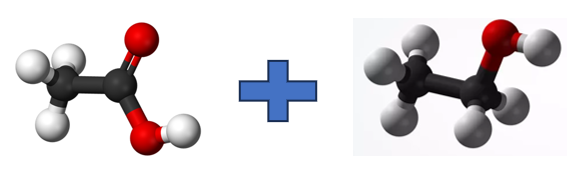
\includegraphics[width=0.86\linewidth]{rasmlar/m_efir.png}\end{center}

\noindent A)~\textsl{3} \hfill B)~\textsl{5} \hfill C)~\textsl{4} \hfill D)~\textsl{2,5}\par
\qsep
\noindent\qn{24.} Aldegid va ketonlar haqida qaysi fikrlar to`g`ri? 1) Aldegidlar qaytarilganda ikkilamchi spirt hosil bo`ladi; 2) Sirka aldegid Kucherov reaksiyasi bilan olinadi; 3) Formaldegid gaz holatda, suvda yaxshi eriydi; 4) Aldegidlar "kumush ko`zgu" reaksiyasini beradi

\noindent A)~\textsl{2, 3, 4} \hfill B)~\textsl{2, 3} \hfill C)~\textsl{1, 2, 3} \hfill D)~\textsl{1, 3}\par
\qsep
\noindent\qn{25.} Karbon kislotalar haqida qaysi fikrlar to`g`ri? 1) Karboksil guruh karbonil va gidroksil guruhlardan iborat; 2) Qattiq suvda sovun yaxshi ko`piklanadi; 3) Olein kislota Br\textsubscript{2} ni biriktiradi; 4) Sirka angidrid ikki molekula sirka kislotadan suv chiqib hosil bo`ladi

\noindent A)~\textsl{1, 2, 3} \hfill B)~\textsl{1, 3, 4} \hfill C)~\textsl{1, 3} \hfill D)~\textsl{2, 4}\par
\qsep
\noindent\qn{26.} 161,2 g tripalmitin natriy ishqori bilan to`liq gidrolizlanganda necha gramm sovun hosil bo`ladi?

\noindent A)~\textsl{55,6} \hfill B)~\textsl{111,2} \hfill C)~\textsl{161,2} \hfill D)~\textsl{166,8}\par
\qsep
\noindent\qn{27.} Quyidagi birikmalardan qaysi biri keton sinfiga kiradi?

\noindent A)~\textsl{C\textsubscript{6}H\textsubscript{5}OH} \hfill B)~\textsl{CH\textsubscript{3}OCH\textsubscript{3}} \hfill C)~\textsl{CH\textsubscript{3}COOH} \hfill D)~\textsl{CH\textsubscript{3}COCH\textsubscript{3}}\par
\qsep
\noindent\qn{28.} Aminlar, aminokislotalar va oqsillar haqida qaysi fikrlar to`g`ri? 1) Glitsin optik faol; 2) Dipeptidda 2 ta peptid bog` bor; 3) Anilin bromli suv bilan oq cho`kma beradi; 4) Aminokislotalar faqat kislotali xossaga ega

\noindent A)~\textsl{2, 4} \hfill B)~\textsl{3, 4} \hfill C)~\textsl{3} \hfill D)~\textsl{1, 2}\par
\qsep
\noindent\qn{29.} 26 g C\textsubscript{2}H\textsubscript{2} dan quyidagi ikki bosqichda C\textsubscript{2}H\textsubscript{6} olinadi: 1) C\textsubscript{2}H\textsubscript{2} + H\textsubscript{2} $\to$ C\textsubscript{2}H\textsubscript{4} (unum 50\%); 2) C\textsubscript{2}H\textsubscript{4} + H\textsubscript{2} $\to$ C\textsubscript{2}H\textsubscript{6} (unum 50\%). Oxirgi mahsulot C\textsubscript{2}H\textsubscript{6} ning \textbf{hajmini (l, n.sh.) toping.}

\noindent A)~\textsl{11,2} \hfill B)~\textsl{5,6} \hfill C)~\textsl{22,4} \hfill D)~\textsl{2,8}\par
\qsep
\noindent\qn{30.} Laboratoriyada vodorod olish uchun qaysi moddalar ishlatiladi?
\noindent A)~\textsl{CaCO\textsubscript{3} + HCl}\par
\noindent B)~\textsl{CH\textsubscript{3}COONa + NaOH (qizdirish)}\par
\noindent C)~\textsl{KMnO\textsubscript{4} (qizdirish)}\par
\noindent D)~\textsl{Zn + HCl}\par
\qsep
\noindent\qn{31.} Rasmdagi usul bilan qaysi moddani eritmadan ajratib olish mumkin?
\begin{center}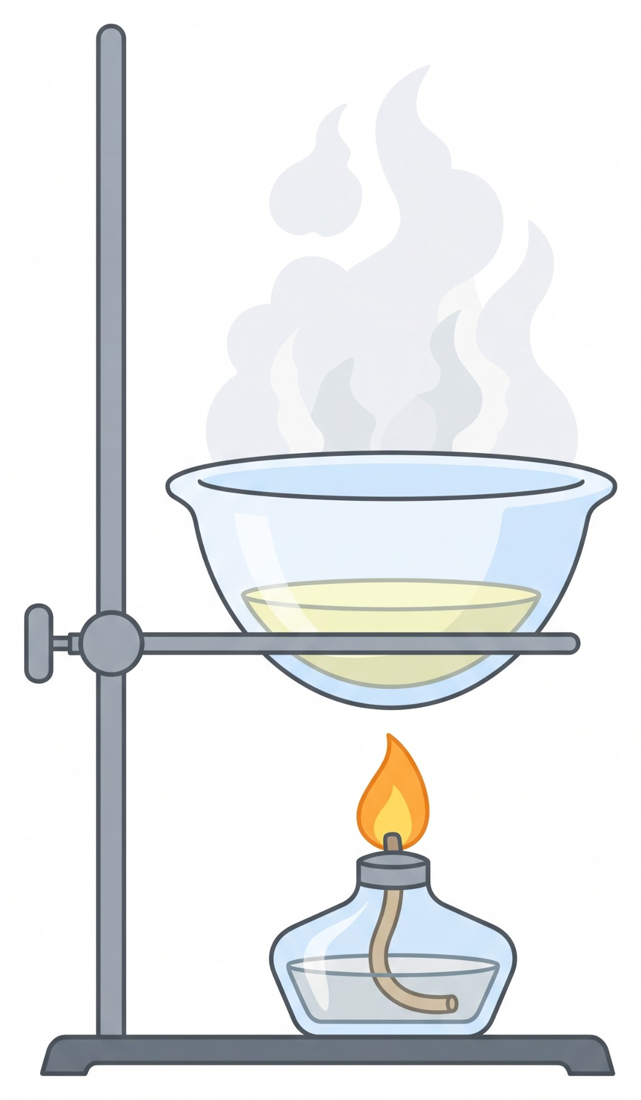
\includegraphics[width=0.86\linewidth]{rasmlar/darslik/d_bugla.png}\end{center}
\noindent A)~\textsl{osh tuzini tuz eritmasidan}\par
\noindent B)~\textsl{kerosinni suvdan}\par
\noindent C)~\textsl{qumni suvdan}\par
\noindent D)~\textsl{suvni osh tuzi eritmasidan (toza holda)}\par
\qsep
\noindent\qn{32.} NaNO\textsubscript{3} ning 50\% li eritmasidan 200 g 10\% li eritma tayyorlash uchun necha gramm suv kerak?

\noindent A)~\textsl{40} \hfill B)~\textsl{200} \hfill C)~\textsl{160} \hfill D)~\textsl{320   ---}\par
\qsep
\end{multicols}
\medskip
\noindent\setlength{\fboxsep}{0pt}\fbox{\begin{tabular}{p{0.74\linewidth}|p{0.2\linewidth}}
\parbox[t]{0.72\linewidth}{\vspace{3pt}\textbf{Topshiriqlar (33--35) va javob variant (A--F)larini o`zaro to`g`ri moslashtiring.} K\textsubscript{2}CO\textsubscript{3} va BaCO\textsubscript{3} dan iborat 60,1 g aralashma mo`l xlorid kislota bilan to`liq reaksiyaga kirishdi.
\vspace{3pt}} & \parbox[t]{0.19\linewidth}{\vspace{3pt}A~\textsl{7,84}\\[3pt]
B~\textsl{52,77}\\[3pt]
C~\textsl{255,5}\\[3pt]
D~\textsl{11,76}\\[3pt]
E~\textsl{6,27}\\[3pt]
F~\textsl{204,4}}\\ \hline
\parbox[t]{0.72\linewidth}{\vspace{2pt}\textbf{33. Ajralgan gaz hajmini (l, n.sh.) aniqlang.}\vspace{2pt}} & \\ \hline
\parbox[t]{0.72\linewidth}{\vspace{2pt}\textbf{34. Aralashmani to`liq eritish uchun sarflangan 10\% li HCl eritmasining massasini (g) aniqlang (M(HCl) = 36,5 g/mol).}\vspace{2pt}} & \\ \hline
\parbox[t]{0.72\linewidth}{\vspace{2pt}\textbf{35. Reaksiyadan so`ng eritmadagi tuzlar umumiy massasini (g) aniqlang.}\vspace{2pt}} & 
\end{tabular}}
\par\bigskip
\noindent\qn{36.} K\textsubscript{2}Cr\textsubscript{2}O\textsubscript{7} + FeSO\textsubscript{4} + H\textsubscript{2}SO\textsubscript{4} $\to$ Cr\textsubscript{2}(SO\textsubscript{4})\textsubscript{3} + Fe\textsubscript{2}(SO\textsubscript{4})\textsubscript{3} + K\textsubscript{2}SO\textsubscript{4} + H\textsubscript{2}O reaksiya tenglamasini tenglang va barcha koeffitsiyentlar \textbf{yig`indisini aniqlang.}
\javob\qsep
\noindent\qn{37.} 5,4 g Al reaksiyaga kirishdi (2Al + 6HCl $\to$ 2AlCl\textsubscript{3} + 3H\textsubscript{2}). Ajralgan H\textsubscript{2} \textbf{hajmini (l, n.sh.) hisoblang} (unum 80\%).
\javob\qsep
\noindent\qn{38.} Al, Fe va Cu dan iborat aralashma mo`l NaOH eritmasi bilan ta'sirlashganda 6,72 l (n.sh.) vodorod ajraldi; xuddi shunday massadagi aralashma mo`l HCl bilan ta'sirlashganda 11,2 l (n.sh.) vodorod ajraldi, erimay qolgan qoldiq (mis) massasi 6,4 g. Aralashmaning dastlabki \textbf{massasini (g) toping.}
\javob\qsep
\noindent\qn{39.} 180 g glyukoza spirtli bijg`ish natijasida etanolga (unum 80\%), hosil bo`lgan etanol esa sirka kislotagacha (unum 75\%) aylantirildi. Olingan kislotani to`liq neytrallash uchun NaOH ning \textbf{massasini (g) toping.}
\javob\qsep
\noindent\qn{40.} Polivinilxlorid polimerining (polimerlanish darajasi 1000) 62,5 g namunasini olish uchun polimerlanish unumi 50\% bo`lganda qancha monomer (C\textsubscript{2}H\textsubscript{3}Cl) kerak (g)?
\javob\qsep
\par\bigskip\begin{center}\textbf{\fontsize{13}{15}\selectfont YOZMA ISH}\end{center}
\noindent\qn{41.} \textbf{Topshiriqni bajarish jarayonida barcha reaksiya tenglamalarini yozing. Miqdoriy va arifmetik hisoblashlarni (unga asos bo`lgan usul yoki formulani ko`rsatgan holda) uzviy ketma-ketlikda bajaring.}\par\smallskip
2 l hajmli idishda N\textsubscript{2} + 3H\textsubscript{2} $\rightleftarrows$ 2NH\textsubscript{3} reaksiyasi muvozanat holatiga keldi. Muvozanatda idishda 4 mol N\textsubscript{2}, 4 mol H\textsubscript{2} va 8 mol NH\textsubscript{3} bor.\par
\noindent 1)Muvozanat konstantasini (K) hisoblang.\par
\noindent 2)Azot va vodorodning boshlang`ich konsentratsiyalarini (mol/l) aniqlang. H\textsubscript{2} ning boshlang`ich massasini (g) ham toping.\par
\noindent 3)Vodorodning necha foizi reaksiyaga kirishgan?\par
\noindent 4)Hosil bo`lgan ammiakning hammasi 800 g suvda eritildi. Eritmadagi ammiakning massa ulushini (\%) hisoblang. Ajralgan NH\textsubscript{3} hajmini (l, n.sh.) ham toping.\par
\noindent 5)Shu eritmani (NH\textsubscript{4})\textsubscript{2}SO\textsubscript{4} hosil bo`lguncha neytrallash uchun 20\% li H\textsubscript{2}SO\textsubscript{4} eritmasidan necha gramm kerak? Idish hajmi 2 marta kamaytirilsa, to`g`ri reaksiya tezligi (elementar deb hisoblang) necha marta ortadi?\par
\diqqat{Mazkur topshiriq kengaytirilgan javobni talab etib, uning yechilish usuli va shu usul asosidagi barcha hisoblash amallari javoblar varaqasida aks etishi lozim.}\qsep
\noindent\qn{42.} Quyidagi o`zgarishlar zanjirida \textit{X}, \textit{Y}, \textit{Z} noma'lum organik moddalar:\par
\[\setlength{\fboxsep}{0pt}\text{CaC\textsubscript{2}}\xrightarrow{\text{H\textsubscript{2}O}}\text{\textit{X}}\xrightarrow{\text{H\textsubscript{2}O, Hg\textsuperscript{2+}}}\text{\textit{Y}}\xrightarrow{\text{Ag\textsubscript{2}O, NH\textsubscript{3}}}\text{\textit{Z}}\xrightarrow{\text{Cl\textsubscript{2}, P}}\text{ClCH\textsubscript{2}COOH}\]
\noindent 1)CaC\textsubscript{2} $\to$ \textit{X} : reaksiya tenglamasini yozing; hosil bo`lgan moddani nomlang.\par
\noindent 2)\textit{X} $\to$ \textit{Y} : reaksiya tenglamasini yozing; hosil bo`lgan moddani nomlang.\par
\noindent 3)\textit{Y} $\to$ \textit{Z} : reaksiya tenglamasini yozing; hosil bo`lgan moddani nomlang.\par
\noindent 4)\textit{Z} $\to$ ClCH\textsubscript{2}COOH : reaksiya tenglamasini yozing; hosil bo`lgan moddani nomlang.\par
\diqqat{Mazkur topshiriq kengaytirilgan javobni talab etib, uning yechilish usuli va shu usul asosidagi barcha hisoblash amallari javoblar varaqasida aks etishi lozim.}\qsep
\noindent\qn{43.} \textbf{Topshiriqni bajarish jarayonida barcha reaksiya tenglamalarini yozing. Miqdoriy va arifmetik hisoblashlarni (unga asos bo`lgan usul yoki formulani ko`rsatgan holda) uzviy ketma-ketlikda bajaring.}\par\smallskip
Uch probirkada (\textit{X}, \textit{Y}, \textit{Z}) natriy yoki kaliy tuzlarining eritmalari bor: Na\textsubscript{2}CO\textsubscript{3}, Na\textsubscript{3}PO\textsubscript{4}, NaBr (tartibsiz). Har bir eritmaga reagentlar ta'sir ettirildi, kuzatuvlar jadvalda:\par
\begin{center}
\renewcommand{\arraystretch}{1.15}
\begin{tabular}{|c|c|c|c|}\hline
\textbf{Reagent} & \textbf{\textit{X}} & \textbf{\textit{Y}} & \textbf{\textit{Z}} \\ \hline
AgNO\textsubscript{3} & och sariq cho`kma (AgBr) & oq-sarg`ish cho`kma & sariq cho`kma (Ag\textsubscript{3}PO\textsubscript{4}) \\ \hline
BaCl\textsubscript{2} & --- & oq cho`kma (BaCO\textsubscript{3}) & oq cho`kma \\ \hline
HCl & --- & gaz (CO\textsubscript{2}) ajraladi & --- \\ \hline
\end{tabular}
\end{center}
\noindent 1)\textit{X}, \textit{Y}, \textit{Z} probirkalardagi moddalarni aniqlang va kuzatilgan reaksiyalarning ionli tenglamalarini yozing.\par
\noindent 2)\textit{X} probirkadagi tuz 0,2 mol miqdorda olingan. Unga mo`l AgNO\textsubscript{3} qo`shilganda hosil bo`lgan cho`kma massasini (g) toping.\par
\noindent 3)Uchala eritmaning har biriga 0,2 mol dan solingan bo`lsa, mo`l AgNO\textsubscript{3} qo`shilganda hosil bo`ladigan barcha cho`kmalarning umumiy massasini (g) toping (ularning formulalarini yozing).\par
\noindent 4)Eritmalarda kuzatilgan hodisalarni (cho`kma yoki gaz hosil bo`lishi) tushuntiring: qaysi ion qaysi reagent bilan qanday birikma hosil qiladi? Shu usul bilan ionlarni aniqlash qoidasini yozing.\par
\noindent 5)Uchala eritmaning har biriga 0,2 mol dan solingan. AgNO\textsubscript{3} bilan cho`kadigan ionlarni to`liq cho`ktirish uchun 10\% li AgNO\textsubscript{3} eritmasidan necha gramm kerak?\par
\diqqat{Mazkur topshiriq kengaytirilgan javobni talab etib, uning yechilish usuli va shu usul asosidagi barcha hisoblash amallari javoblar varaqasida aks etishi lozim.}\qsep
\newpage
\noindent\textbf{\fontsize{13}{15}\selectfont Nazorat testi}\ \textit{$\cdot$ 11-variant}\hfill \textbf{Javoblar kaliti}\par\smallskip\hrule\smallskip
\textit{Faqat o`qituvchi uchun.}\par\medskip
\noindent\textbf{1--32-savollar}\par\smallskip
\noindent\begin{tabular}{|c|c|c|c|c|c|c|c|c|c|c|c|c|c|c|c|}\hline
\textbf{1} & \textbf{2} & \textbf{3} & \textbf{4} & \textbf{5} & \textbf{6} & \textbf{7} & \textbf{8} & \textbf{9} & \textbf{10} & \textbf{11} & \textbf{12} & \textbf{13} & \textbf{14} & \textbf{15} & \textbf{16}\\\hline
\textsl{A} & \textsl{C} & \textsl{A} & \textsl{C} & \textsl{C} & \textsl{B} & \textsl{A} & \textsl{C} & \textsl{C} & \textsl{D} & \textsl{B} & \textsl{A} & \textsl{A} & \textsl{D} & \textsl{B} & \textsl{D}\\\hline
\textbf{17} & \textbf{18} & \textbf{19} & \textbf{20} & \textbf{21} & \textbf{22} & \textbf{23} & \textbf{24} & \textbf{25} & \textbf{26} & \textbf{27} & \textbf{28} & \textbf{29} & \textbf{30} & \textbf{31} & \textbf{32}\\\hline
\textsl{B} & \textsl{B} & \textsl{D} & \textsl{B} & \textsl{D} & \textsl{A} & \textsl{C} & \textsl{A} & \textsl{B} & \textsl{D} & \textsl{D} & \textsl{C} & \textsl{B} & \textsl{D} & \textsl{A} & \textsl{C}\\\hline
\end{tabular}\par\medskip
\noindent\textbf{33--35-savollar}\par\smallskip
\noindent\begin{tabular}{|c|c|c|}\hline \textbf{No} & \textbf{Javob} & \textbf{Qiymat}\\\hline
33 & \textsl{A} & 7,84\\\hline
34 & \textsl{C} & 255,5\\\hline
35 & \textsl{B} & 52,77\\\hline
\end{tabular}\par\medskip
\noindent\textbf{36--40-savollar}\par\smallskip
\noindent\begin{tabular}{|c|c|}\hline \textbf{No} & \textbf{To`g`ri javob}\\\hline
36 & 26\\\hline
37 & 5,38\\\hline
38 & 23\\\hline
39 & 48\\\hline
40 & 125\\\hline
\end{tabular}\par\medskip
\noindent\textbf{41--43-topshiriqlar: javoblar}\par\smallskip
\noindent\textbf{41-topshiriq.}\par
\noindent 1) 1\par
\noindent 2) 4 mol/l; 8 mol/l; 32 g\par
\noindent 3) 75\%\par
\noindent 4) 14,53\%; 179,2 l\par
\noindent 5) 1960 g; 16 marta\par
\noindent\textbf{42-topshiriq.}\par
\noindent 1) CaC\textsubscript{2} + H\textsubscript{2}O $\to$ C\textsubscript{2}H\textsubscript{2} (asetilen)\par
\noindent 2) C\textsubscript{2}H\textsubscript{2} + H\textsubscript{2}O, Hg\textsuperscript{2+} $\to$ CH\textsubscript{3}CHO (sirka aldegid (etanal))\par
\noindent 3) CH\textsubscript{3}CHO + Ag\textsubscript{2}O, NH\textsubscript{3} $\to$ CH\textsubscript{3}COOH (sirka kislota)\par
\noindent 4) CH\textsubscript{3}COOH + Cl\textsubscript{2}, P $\to$ ClCH\textsubscript{2}COOH (xlorsirka kislota)\par
\noindent\textbf{43-topshiriq.}\par
\noindent 1) \textit{X} -- NaBr, \textit{Y} -- Na\textsubscript{2}CO\textsubscript{3}, \textit{Z} -- Na\textsubscript{3}PO\textsubscript{4}. Ionli tenglamalar: Ag\textsuperscript{+} + Br\textsuperscript{$-$} $\to$ AgBr$\downarrow$; Ag\textsuperscript{+} + PO\textsubscript{4}\textsuperscript{3$-$} $\to$ Ag\textsubscript{3}PO\textsubscript{4}$\downarrow$; CO\textsubscript{3}\textsuperscript{2$-$} + 2H\textsuperscript{+} $\to$ CO\textsubscript{2}$\uparrow$ + H\textsubscript{2}O\par
\noindent 2) 37,6 g\par
\noindent 3) 176,6 g\par
\noindent 4) Cl\textsuperscript{$-$} + Ag\textsuperscript{+} $\to$ AgCl (oq), Br\textsuperscript{$-$} $\to$ AgBr (och sariq), I\textsuperscript{$-$} $\to$ AgI (sariq), SO\textsubscript{4}\textsuperscript{2$-$} + Ba\textsuperscript{2+} $\to$ BaSO\textsubscript{4} (oq), CO\textsubscript{3}\textsuperscript{2$-$} + H\textsuperscript{+} $\to$ CO\textsubscript{2} (gaz). Har \par
\noindent 5) 2040 g\par
\par\bigskip\noindent\textbf{Mavzular taqsimoti}\par\smallskip
{\small\noindent\begin{longtable}{|c|p{7.2cm}|p{5.4cm}|c|}\hline \textbf{No} & \textbf{Mavzu} & \textbf{Tekshiriladigan ko`nikma} & \textbf{Ball}\\\hline
1 & 8-sinf (ortiqcha modda masalasi) & Hisoblash va masala yechish & 1\\\hline
2 & Tirkashev III bob (kristallogidrat) & Hisoblash va masala yechish & 1\\\hline
3 & Tirkashev III bob (eritmalar, jadval) & Jadval tahlili & 1\\\hline
4 & 8-sinf (kimyoviy bog`lanish turlari, jadval) & Jadval tahlili & 1\\\hline
5 & 7-sinf (Avogadro) & Hisoblash va masala yechish & 1\\\hline
6 & 7-sinf; Tirkashev (kristallogidrat) & Hisoblash va masala yechish & 1\\\hline
7 & 11-sinf 8-bob; Tirkashev \textit{V} bob (elektroliz) & Bilim va tushunish & 1\\\hline
8 & 11-sinf 1-bob (yadro reaksiyalari) & Bilim va tushunish & 1\\\hline
9 & 9-sinf (gidroliz); Tirkashev IV bob & Bilim va tushunish & 1\\\hline
10 & 10-sinf \S{}17 & Bilim va tushunish & 1\\\hline
11 & 8-sinf (ionlanish energiyasi, grafik) & Grafik tahlili & 1\\\hline
12 & 11-sinf 1-bob (yadro reaksiyalari) & Bilim va tushunish & 1\\\hline
13 & 7-sinf (valentlik) & Bilim va tushunish & 1\\\hline
14 & Tashev (nodir gazlar); 8-sinf & Bilim va tushunish & 1\\\hline
15 & Tashev (nitratlar) & Bilim va tushunish & 1\\\hline
16 & 9-sinf; Tirkashev (S/SO\textsubscript{2}/H\textsubscript{2}SO\textsubscript{4}, hisob) & Hisoblash va masala yechish & 1\\\hline
17 & Tashev (nitratlar termik parchalanishi) & Hisoblash va masala yechish & 1\\\hline
18 & 9-sinf; Tirkashev (P/C/Si, hisob) & Hisoblash va masala yechish & 1\\\hline
19 & 9-sinf; Tirkashev (galogenlar, hisob) & Hisoblash va masala yechish & 1\\\hline
20 & 10-sinf (alkan, hisob) & Hisoblash va masala yechish & 1\\\hline
21 & 10-sinf (alken, hisob) & Hisoblash va masala yechish & 1\\\hline
22 & 10-sinf \S{}15 (asetilen olinishi) & Hisoblash va masala yechish & 1\\\hline
23 & 10-sinf \S{}17, \S{}28 & Rasm bo`yicha tahlil & 1\\\hline
24 & 10-sinf (mavzuga oid paragraflar); Abdusamatov & Bilim va tushunish & 1\\\hline
25 & 10-sinf (mavzuga oid paragraflar); Abdusamatov & Bilim va tushunish & 1\\\hline
26 & 10-sinf \S{}29 (yog`lar, sovunlanish) & Hisoblash va masala yechish & 1\\\hline
27 & 10-sinf (organik birikmalar sinflari) & Bilim va tushunish & 1\\\hline
28 & 10-sinf (mavzuga oid paragraflar); Abdusamatov & Bilim va tushunish & 1\\\hline
29 & 10-sinf (ikki bosqichli hisob) & Hisoblash va masala yechish & 1\\\hline
30 & 9--10-sinf (laboratoriya usullari bilan gaz olish) & Bilim va tushunish & 1\\\hline
31 & 7-sinf (12-rasm) & Rasm bo`yicha tahlil & 1\\\hline
32 & Tirkashev III bob (eritmalar) & Hisoblash va masala yechish & 1\\\hline
33--35 & Aralash masala (moslashtirish) & Ko`p bosqichli hisob & 3\\\hline
36--40 & Qisqa javobli masalalar & Hisoblash & 5\\\hline
41--43 & Yozma ish & Usul va hisob (M, A) & 75\\\hline
\end{longtable}}
\end{document}
